
\section{Type Definitions}

\begin{table}[ht]
\centering
 \resizebox{0.6\textwidth}{!}{
\begin{tabular}{|lll|c|lll|}
  \hline
 & denotion & classification & & & denotion & classification \\ 
  \hline
  0 & L-LLL & selfish &  &   41 & M-MMH & conditional \\ 
  1 & L-LLM & conditional &  &   42 & M-MHL & humped \\ 
  2 & L-LLH & conditional &  &   43 & M-MHM & humped \\ 
  3 & L-LML & humped &  &   44 & M-MHH & conditional \\ 
  4 & L-LMM & conditional &  &   45 & M-HLL & other \\ 
  5 & L-LMH & perf-conditional &  &   46 & M-HLM & other \\ 
  6 & L-LHL & humped &  &   47 & M-HLH & other \\ 
  7 & L-LHM & humped &  &   48 & M-HML & other \\ 
  8 & L-LHH & conditional &  &   49 & M-HMM & other \\ 
  9 & L-MLL & other &  &   50 & M-HMH & other \\ 
  10 & L-MLM & other &  &   51 & M-HHL & other \\ 
  11 & L-MLH & other &  &   52 & M-HHM & unconditional \\ 
  12 & L-MML & other &  &   53 & M-HHH & unconditional \\ 
  13 & L-MMM & unconditional &  &   54 & H-LLL & selfish \\ 
  14 & L-MMH & conditional &  &   55 & H-LLM & conditional \\ 
  15 & L-MHL & humped &  &   56 & H-LLH & conditional \\ 
  16 & L-MHM & humped &  &   57 & H-LML & humped \\ 
  17 & L-MHH & conditional &  &   58 & H-LMM & conditional \\ 
  18 & L-HLL & other &  &   59 & H-LMH & perf-conditional \\ 
  19 & L-HLM & other &  &   60 & H-LHL & humped \\ 
  20 & L-HLH & other &  &   61 & H-LHM & humped \\ 
  21 & L-HML & other &  &   62 & H-LHH & conditional \\ 
  22 & L-HMM & other &  &   63 & H-MLL & other \\ 
  23 & L-HMH & other &  &   64 & H-MLM & other \\ 
  24 & L-HHL & other &  &   65 & H-MLH & other \\ 
  25 & L-HHM & unconditional &  &   66 & H-MML & other \\ 
  26 & L-HHH & unconditional &  &   67 & H-MMM & unconditional \\ 
  27 & M-LLL & selfish &  &   68 & H-MMH & conditional \\ 
  28 & M-LLM & conditional &  &   69 & H-MHL & humped \\ 
  29 & M-LLH & conditional &  &   70 & H-MHM & humped \\ 
  30 & M-LML & humped &  &   71 & H-MHH & conditional \\ 
  31 & M-LMM & conditional &  &   72 & H-HLL & other \\ 
  32 & M-LMH & perf-conditional &  &   73 & H-HLM & other \\ 
  33 & M-LHL & humped &  &   74 & H-HLH & other \\ 
  34 & M-LHM & humped &  &   75 & H-HML & other \\ 
  35 & M-LHH & conditional &  &   76 & H-HMM & other \\ 
  36 & M-MLL & other &  &   77 & H-HMH & other \\ 
  37 & M-MLM & other &  &   78 & H-HHL & other \\ 
  38 & M-MLH & other &  &   79 & H-HHM & unconditional \\ 
  39 & M-MML & other &  &   80 & H-HHH & unconditional \\ 
  40 & M-MMM & unconditional &  &  & & \\ \hline 
\end{tabular}
}
\caption{All Possible Types and Their Classifications}
\label{tbl:evo-alltypes}
\end{table}



\section{Additional Data}
\label{sec:evo-additional}
\begin{figure}[H]
\begin{center}
    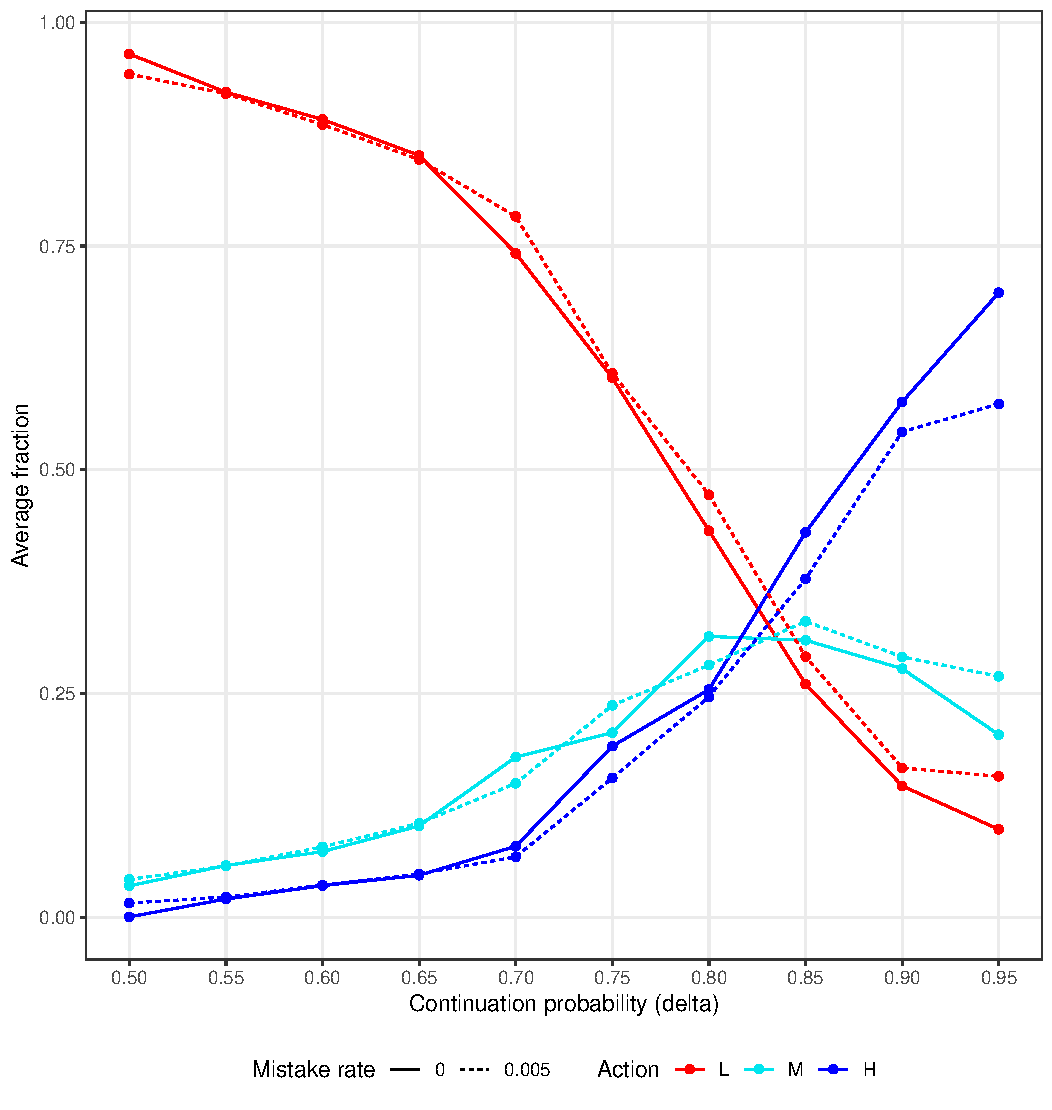
\includegraphics[width=0.8\linewidth]{img/actions_over_delta_with_mistakes.pdf}
    \caption{Comparison of Actions with and without mistakes.}
	\label{fig:mistake-comparision}
\end{center}
\end{figure}


\begin{figure}[H]
\begin{center}
    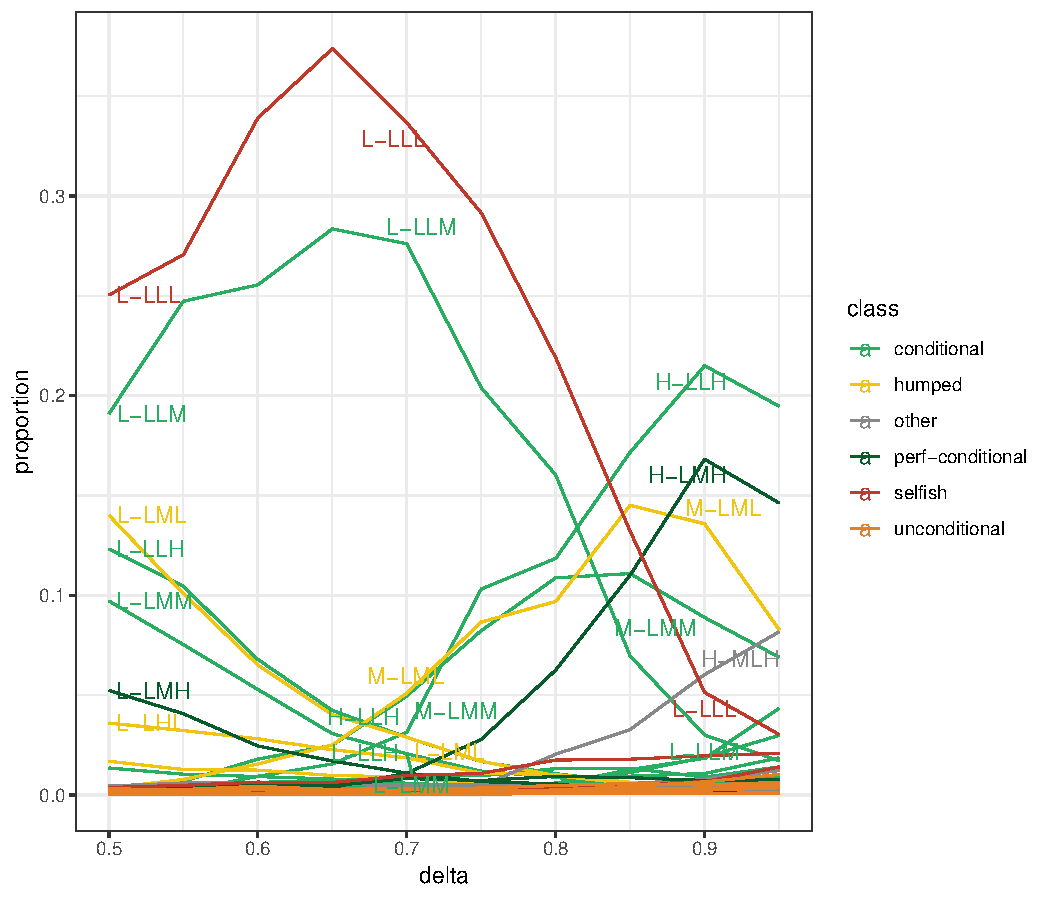
\includegraphics[width=0.8\linewidth]{img/all_types_t05.pdf}
    \caption{All types' performance for different continuation probabilities.}
	\label{fig:alltypes}
\end{center}
\end{figure}


%%% Local Variables:
%%% mode: latex
%%% TeX-master: "../main"
%%% End:
